\documentclass[11pt]{article}
\usepackage[utf8]{inputenc}
\usepackage{graphicx}
\usepackage{pgf-pie}
\usepackage{geometry}
\geometry{a4paper}
\usepackage{caption}
\usepackage{changepage}
\usepackage{longtable}
\setcounter{secnumdepth}{0}
\setlength{\parskip}{\baselineskip}
\setlength{\parindent}{0pt}

\usepackage{filecontents}
\begin{filecontents}{testbib.bib}
@inproceedings{1,
author={Endestad Tor and Torgersen Leila},
year={2003},
title={Computer games and violence: Is there really a connection?},
isbn={ISSN 2342-9666},
booktitle={DiGRA \&\#3903 - Proceedings of the 2003 DiGRA International Conference: Level Up},
url={http://www.digra.org/wp-content/uploads/digital-library/05163.54594.pdf}
}

@article{2,
author = {Gotterbarn, Donald and Moor, James},
year = {2009},
month = {12},
pages = {27-42},
title = {Virtual decisions: video game ethics, Just Consequentialism, and ethics on the fly},
volume = {39},
journal = {ACM Sigcas Computers and Society},
doi = {10.1145/1713066.1713068}
}

@inproceedings{3,
author = {Ashbarry, Louise and Geelan, Ben and de Salas, Kristy and Lewis, Ian},
year = {2016},
month = {10},
pages = {44-52},
title = {Blood and Violence: Exploring the Impact of Gore in Violent Video Games},
doi = {10.1145/2967934.2968111}
}

@article{4,
author = {Anderson, Craig},
year = {2004},
month = {03},
pages = {113-22},
title = {An update on the effects of playing violent video games},
volume = {27},
journal = {Journal of adolescence},
doi = {10.1016/j.adolescence.2003.10.009}
}

@article{5,
author = {Carnagey, Nicholas and Anderson, Craig},
year = {2004},
month = {03},
pages = {1-18},
title = {Violent video game exposure and aggression: A literature review},
volume = {45},
journal = {Minerva Psichiatrica}
}

@article{6,
author = {Anderson, Craig and Ford, Catherine},
year = {1986},
month = {12},
pages = {390-402},
title = {Affect of the Game Player Short-Term Effects of Highly and Mildly Aggressive Video Games},
volume = {12},
journal = {Personality and Social Psychology Bulletin},
doi = {10.1177/0146167286124002}
}

@article{7,
author = {Egli E. A., Meyers L. S.},
year = {1984},
pages = {309-312},
title = {The role of video game playing in adolescent life: Is there a reason to be concerned?},
volume = {22},
journal = {Bulletin of the Psychonomic Society},
doi = {10.3758/BF03333828}
}

@article{8,
author = {Wiegman, Oene and van Schie, Emil G. M.},
title = {Video game playing and its relations with aggressive and prosocial behaviour},
journal = {British Journal of Social Psychology},
volume = {37},
number = {3},
pages = {367-378},
doi = {10.1111/j.2044-8309.1998.tb01177.x},
url = {https://onlinelibrary.wiley.com/doi/abs/10.1111/j.2044-8309.1998.tb01177.x},
eprint = {https://onlinelibrary.wiley.com/doi/pdf/10.1111/j.2044-8309.1998.tb01177.x},
year = {1998}
}
\end{filecontents}
\usepackage[style=authoryear,backend=bibtex]{biblatex}
\bibliography{testbib}

\title{A Meta-Analysis of Violent Trends as a Result of Violent Media}
\author{Evan Bryer, William Zhang}
\date{}

\begin{document}
\nocite{*}
\maketitle
\begin{abstract}
Violence in video games has been present since the inception of the medium, and for decades it has been under scrutiny. The debate over the contribution violent media makes to real life violence has been especially pertinent in political discussions lately, as an increase in mass shootings has been attributed to video games by multiple parties. The claims made by both sides of the debate, however, are often unsubstantiated by empirical evidence or academic findings. It may be possible to remedy this by collecting data and conclusions from multiple studies that have been performed, both qualitative and quantitative, so a more precise conclusion can be drawn on the contributions violent media, particularly video games. make on the psychological state of its consumers. To these ends, this paper will collect peer reviewed studies from multiple sources, and compare the conclusions that they have drawn. One finding that has been clear through many of the studies is a short term increase of aggression, though the causal relationship between this and video games is dubious at best.
\end{abstract}
\section{Introduction}

Media, since its inception, has been a form of entertainment that has been able to encompass a large range of genres. From romance, to comedy, to action, to slasher, there have been movies, television shows, and video games that have been able to appeal to any fashion of person. However, the interactivity provided by the last of those forms of media have given rise to great concerns by parents, legislators, educators, and the general public. The question has been asked for many years, “Do violent video games cause real world violence?” and to that end, many different studies have been performed. The goal of this meta-analysis is to explore some of these studies that have been done, and try to find overarching trends present in them in attempts to draw evidence on this matter. 

As early as 1993, the United States Congress had been made aware of the concerns surrounding video games. In hopes of getting government regulation, Senator Herb Kohl and Senator Joe Lieberman used scenes of violence from Mortal Kombat and Night Trap as evidence to video games being too violent for children. These hearings brought about the creation of the Entertainment Software Rating Board, or ESRB, in hopes of moderating video game content, and preventing violent video games from getting in the hands of children. In the present day, however, it seems many children and teens get their hands on violent games, whether or not they fall into the age range the games are advertised towards. Because of this, studies working to find a connection, or lack thereof, between violent video games and real life violent tendencies are more relevant than ever.

\section{Method} 
To gather the sources this paper would analyze, the Digital Games Research Association (DIGRA) digital library, as well as the library of the Association for Computing Machinery (ACM) were consulted. The intention for pulling from a minimum of two journals was to avoid the potential for a singular journal publishing results skewed towards a single conclusion. To further these ends, studies from both psychological journals and the Journal of Adolescence had also been gathered for analysis. Following the completion of studies being gathered, and confirmation of the studies’ peer reviewed status, the conclusion and data sections were scoured for overarching results, and the data that contributed to the conclusion that had been drawn. For studies that provided the number of participants, this value was also noted, to be used during our analysis.

\section{Results}
Of the research papers gathered to create this meta-analysis, the conclusions can be separated into the broad categories of “No Effects Observed”, “Only Short Term Negative Effects Observed”, “Long Term Negative Effects Observed” and “Insufficient Evidence for Conclusion”. To be delegated as having insufficient evidence, a study must either fail to make conclusions based on provided data, instead postulating the conclusions based on ethical or general hypotheses. When separated (fig. 1), the most common result is the observation of a short term increase in aggressive behavior.

When the collected studies are analyzed based on the number of participants in the study as opposed to only observing the conclusions drawn (fig 3.), a much higher bias towards short term effects can be found. More significantly, however, long term negative effects are much more represented based on participants in the studies when compared to no effects being observed. While this does not disqualify the studies finding a lack of correlation between aggression and video game consumption, the small number of participants in these studies does bring into question the scalability of some of the findings.

\begin{longtable}{|p{2.55cm}|p{2.55cm}|p{2.55cm}|p{2.55cm}|p{2.55cm}|}
\captionsetup{labelformat=empty}
\caption{Fig. 1. Studies categorized by conclusion.}\\
\hline
\textbf{Title}&\textbf{No Effect Observed}&\textbf{Only Short Term Negative Effects Observed}&\textbf{Long Term Negative Effects Observed}&\textbf{Insufficient Evidence for Conclusion}\\
\hline
Computer games and violence: Is there really a connection?&&Yes: Age was an important factor in determining effect.&&\\
\hline
Virtual Decisions: Video Game Ethics, Just Consequentialism, and Ethics on the Fly&&&&Not an experimental study, therefore no conclusions can be drawn.\\
\hline
Blood and Violence: Exploring the Impact of Gore in Violent Video Games&Yes: no significant correlation observed.&&&Potentially not scalable due to small sample size of only 30 participants.\\
\hline
An update on the effects of playing violent video games&&&Yes: A review of multiple studies come to a conesus on it affecting aggressive and antisocial behavior&\\
\hline
Affect of the Game Player Short-Term Effects of Highly and Mildly Aggressive Video Games&&Yes: observes short term increases in aggression, but notes potential problems within methodology&&Potentially not scalable due to small sample sizes in experiments of 55 and 60 respectively\\
\hline
The Role of Video Game Playing in Adolescent Life: Is There Reason to be Concerned?&Yes: No negative social consequences found in relation to playing video games&&&\\
\hline
Video Game Playing and its Relations with Aggressive and Prosocial  Behaviour&&Yes: Students who indicated heavy video game playing showed a negative relationship to prosocial behavior when compared to those indicating mild to no video game playing&&\\
\hline
\end{longtable}

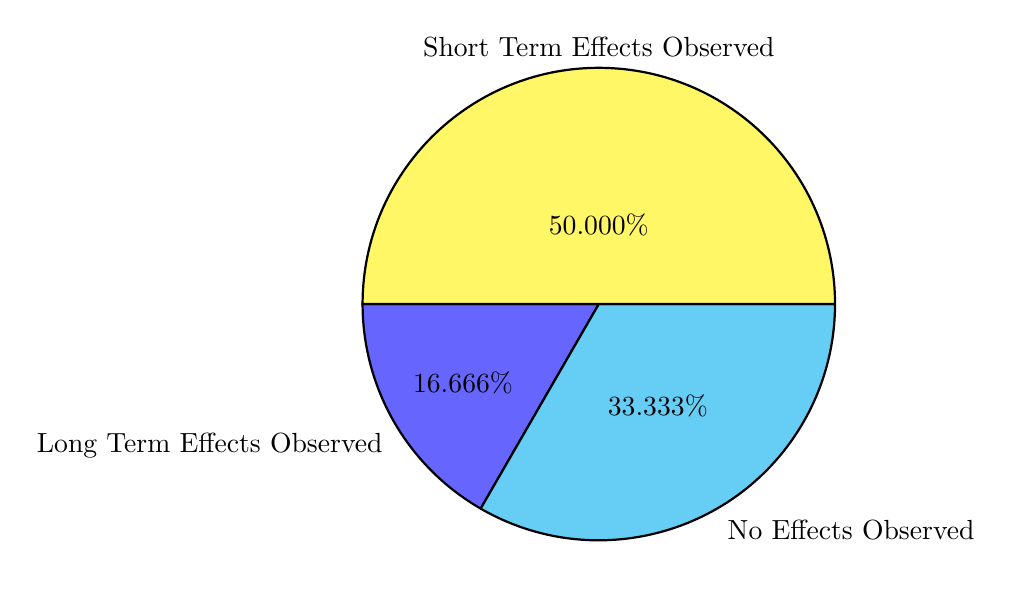
\begin{tikzpicture}
 \pie [rotate=180]
    {16.666/Long Term Effects Observed,
     33.333/No Effects Observed, 50.000/Short Term Effects Observed}
\end{tikzpicture}

\centerline{Fig. 2. Conclusion categorization visualized.}
\begin{adjustwidth}{1in}{1in}
\small{"A pie chart showing the distribution of conclusions as laid out into the three specified overarcing categories. The scale of this is based on the number of studies gathered."}
\end{adjustwidth}

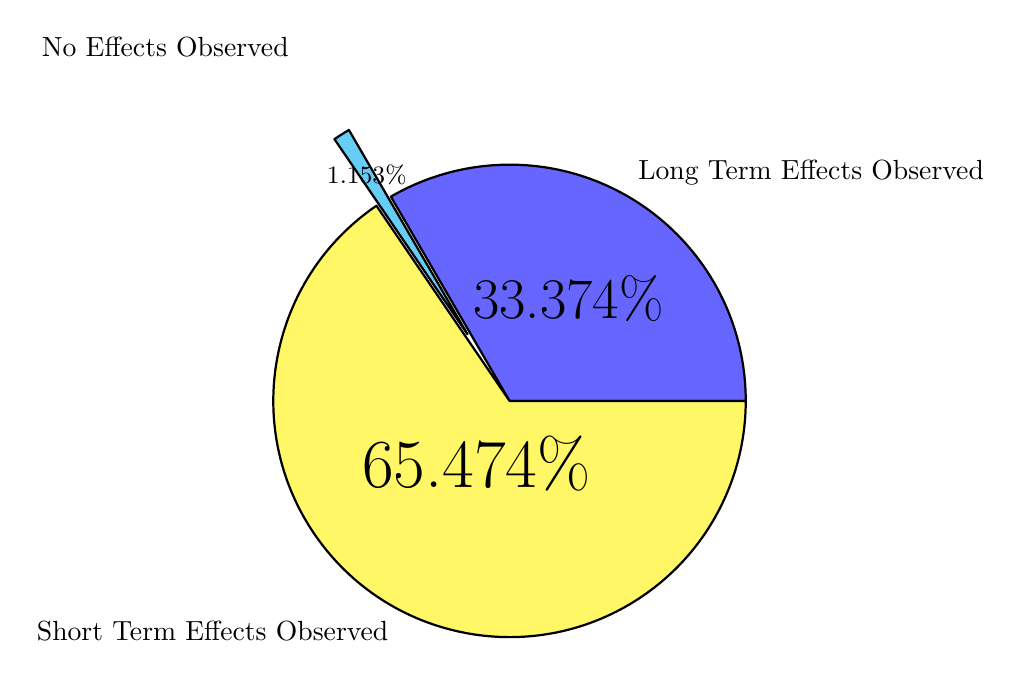
\begin{tikzpicture}
 \pie [ scale font, explode ={0 , 1 , 0}]
    {33.374/Long Term Effects Observed,
     1.153/No Effects Observed, 65.474/Short Term Effects Observed}
\end{tikzpicture}

\centerline{Fig. 3. Conclusions visualized by number of participants in study.}
\begin{adjustwidth}{1in}{1in}
\small{"A pie chart showing the distribution of conclusions as laid out into the three specified overarcing categories, using the number of participants in these studies as the scale. For each study, the conclusion drawn is generalized over the stated number of participants in the study, then charted here to show how this causes the distributions change."}
\end{adjustwidth}

\section{Conclusion}

The majority of the conclusions from the studies we have collected, including when these conclusions are generalized among the participants of the studies, point towards the observed effect of violent video games causing a short term increase in aggressive behaviors. The speculation over the cause of this differs between the multiple studies, however. While some of the negative effects are suggested to be as a result of the observed violence (i.e. Virtual decisions: video game ethics, Just Consequentialism, and ethics on the fly), a study more commonly collaborated by these papers is the competitive atmosphere generated by playing video games to increase psychological arousal. An apparent case of this is within “Computer games and violence: Is there really a connection?”, which includes a portion where Tor Endestad and Leila Torgersen attempt to predict violent behaviour from different genres of video games. This section of the research finds that, just behind first person and action games, the genre of game most likely to predict aggressive behavior is racing games.

The finding that not only violent video games can lead to an increase in violence does point to an alternative explanation for the aggressive behavior. A common theme of many violent video games (e.g. first person shooters, fighting games, and Multiplayer online battle arenas) is a great sense of competition. Points, leaderboards, K/D, and other statistics that are gathered throughout gameplay are often compared and fought over. As is the nature of a competitive atmosphere, where players can see their ego challenged and skill undermined, it reasons that an increase in aggressive behavior can be found for a time even after gameplay finishes, as the increase of stress does not necessarily vanish just as the game finishes.

A potentially disconcerting finding made clear from the participant analysis of each study is the relatively small number of subjects in each of the studies that find no connection between violent video games and aggressive behaviors. Despite having a higher percentage of conclusions pointing towards no connection than pointing to long term effects existing, the studies pointing to long term effects had nearly twenty-nine times more participants. Regardless of the soundness of the methodology or sampling techniques, the small pool of participants does bring into question whether or not the findings of these studies can be considered valid. 

One notable factor that could have potentially skewed the results of our meta-analysis is the much lesser pool of longitudinal, causational studies of violent video game exposure and aggressive behavior over larger periods of time. Because this type of study is far less prevalent than those observing short term effects, it is difficult to attempt to draw a correlation between long term exposure and if it creates a notable increase in aggression after a competitive atmosphere is no longer present. 

An important note to make is that the correlation may not be that of violent video games inspiring aggressive tendencies, but that of those with violent tendencies to prefer the consumption of violent video games. It reasons that consumers will indulge in the genre of media that most suits their tastes, so those predisposed to violence, or those who feel a heightened sense of competitiveness may be particularly drawn to violent, highly competitive video games. This fact further lessens the impact of correlations between violence and video games, as it brings into the question the notion that its the fault of the video games that participants may feel aggressive tendencies.

Overall, the data collected in this meta-analysis points to the potential of a short-term increase of aggressive behavior being correlated to the consumption of violent video games, and other forms of competitive video games. While this does not rebut the possibility of there being long-term ramifications of repeated, copious sessions of playing video games with high amounts of violence, it does suggest that without more causational longitudinal studies, a likely explanation for the increase is a result of the nature of a high stress competitive atmosphere. As such, moderate and balanced consumption of violent media should not be a cause for concern.

\section{Acknowledgements}

This work is partially supported by a grant from the University of South Carolina Magellan Apprentice Program.

\printbibliography

\end{document}